\chapter{Background}\label{chapter:background}
In this chapter we introduce techniques described in Team Description Papers of the \cite{robocup} and papers about Soccer Simulation 2D. In Section \ref{section:DefensiveDeterministic} we present deterministic techniques for defensive agents. Also in this chapter, in Section \ref{section:RLAgents} we show Reinforcement Learning techniques applied to defensive.

\section{Deterministic Agents}\label{section:DefensiveDeterministic}
In this section we shall explain some successful deterministic techniques applied to Soccer Simulation 2D league. Most of them are very useful as baseline or the teams actual defense line.

\subsection{Marlik2011 Defense}
\cite{marlik2011} created one of the best Defensive behaviour presented in the Soccer Simulation 2D League used since then in great teams like Fractals2019, \cite{glidersv2}. It was combined by three high-level actions: Cross Mark, Play\_on Mark and Block. Since they released the code, the RoboCIn team included those actions to their agent and it raised up to 60\% of the successful defenses.

\subsubsection{Cross Mark}
This behaviour occurs when an opponent reaches near one of the defensive corner flags, usually when -36 > Ball-X > -53 and 20 < |Ball-Y| < 34. The main idea of the algorithm is to position the marker between the nearest attacker and the ball to reach the ball faster. When the number of defenders is greater than the attackers, man-to-man marking will be done and the rest of the markers will guard the goal for probable shots. When attackers have an advantage, the three midfielders (usually numbers 6, 7 and 8) will try to mark opponents depending on their stamina. In Figure \ref{fig:crossmark} we can see an example of the behaviour.

\begin{figure}[H]
    \centering
    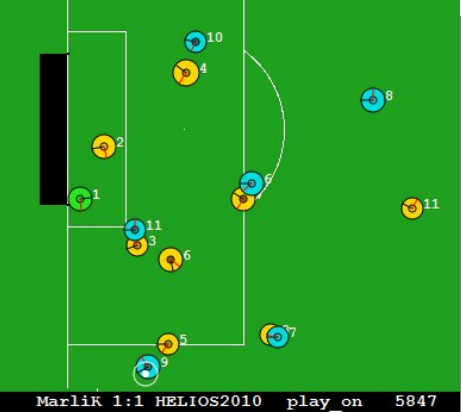
\includegraphics[scale=0.5]{images/cross_mark.png}
    \caption{Cross Mark behaviour. Observe the positioning of numbers 3, 4, 7 and 8 how the get in "front" of the attackers. Image from \cite{marlik2011}.}
    \label{fig:crossmark}
\end{figure}


\subsubsection{Play\_on Mark}
This type of marking is to avoid through passes and it is only applied on defenders, usually numbers 2, 3, 4 and 5. The idea is to disarm the attack when they are trying to break the defense line. Depending on attackers position and the defenders formation, the marker will choose one of the attackers to stay "behind" and then block a possible through pass. In Figure \ref{fig:playonmark} and \ref{fig:playonmark2} we can see examples of the behaviour.

\begin{figure}[H]
    \centering
    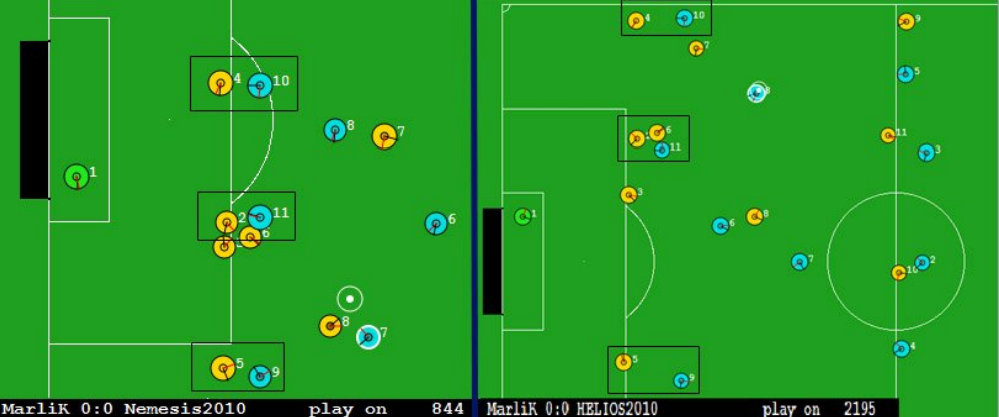
\includegraphics[scale=0.5]{images/play_on_mark.png}
    \caption{Play\_on Mark behaviour. Image from \cite{marlik2011}.}
    \label{fig:playonmark}
\end{figure}

\begin{figure}[H]
    \centering
    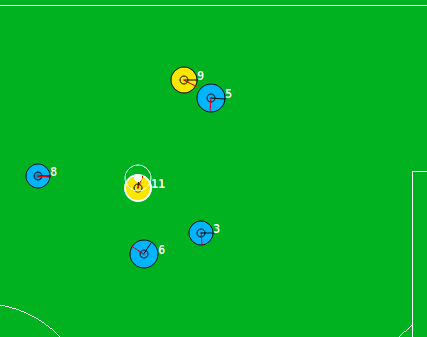
\includegraphics[scale=0.5]{images/play_on_mark2.png}
    \caption{Play\_on Mark behaviour. Observe the positioning of numbers 5 and 3 ready to block a through pass.}
    \label{fig:playonmark2}
\end{figure}

\subsubsection{Block}
Block is the most efficient technique of Marlik2011. Including only it in RoboCIn's code, the behaviour reduced from an average of 7 goals taken from  HELIOS2018 to an average of 2 goals taken. 

It has two important parts: moving to the best block point and decide how to act then. When the defender is the near from the ball, the best block point is calculated by a prediction of opponent's future dribble target. When the agent is too far from the attacker in possession, it marks the nearest opponent, see Figure \ref{fig:block}. Once the agent have reached the best position to block the attack, the defender will decide if it will continue doing the block, intercept the ball or push the attackers back, see Figure \ref{fig:block2}.

\begin{figure}[h]
    \centering
    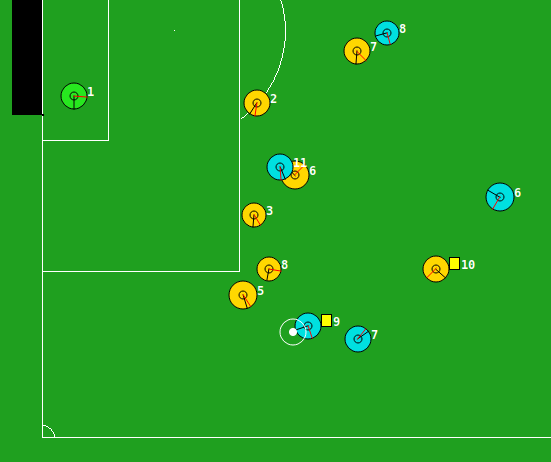
\includegraphics[scale=0.5]{images/block_pass.png}
    \caption{Block behaviour. Observe the yellow team positioning of numbers 6, 7 and 10 ready to block the pass.}
    \label{fig:block}
\end{figure}

\begin{figure}[H]
    \centering
    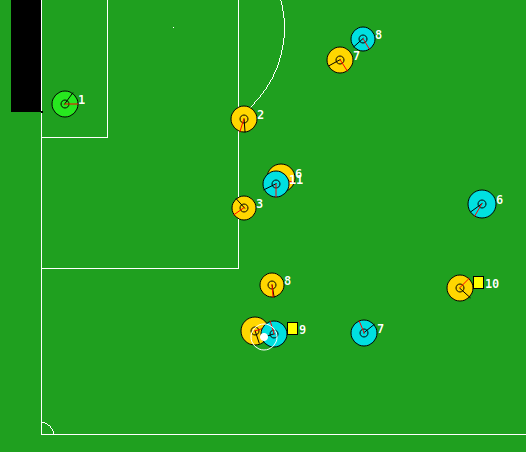
\includegraphics[scale=0.5]{images/marlik_block.png}
    \caption{Block behaviour. Observe the positioning of number 5 going to intercept the ball.}
    \label{fig:block2}
\end{figure}


\subsection{WrightEagle2014 Defense}
The WrightEagle team, \cite{wrighteagle2014}, did an interesting research on defenses areas and ranges. Their algorithm draws defensible areas based on defender formation's position and a number K opponents attackers. K represents how many opponents can represent better the attack or the most valuated weights calculated by the algorithm. The K weights are summed up and normalized and then the area with greater weight is chosen to be defended. In figure \ref{fig:defensenet} we can see an example of defense nets.

\subsection{Gliders2d Defense}
\cite{glidersv1} showed a simple defense improving with Gliders2D that caused their winning of RoboCup 2016. They fine tuned the pressing variable considering the role of the agent, the position of the ball and the opponent team, see Figure \ref{fig:gliderscode}. 

\begin{figure}[H]
    \centering
    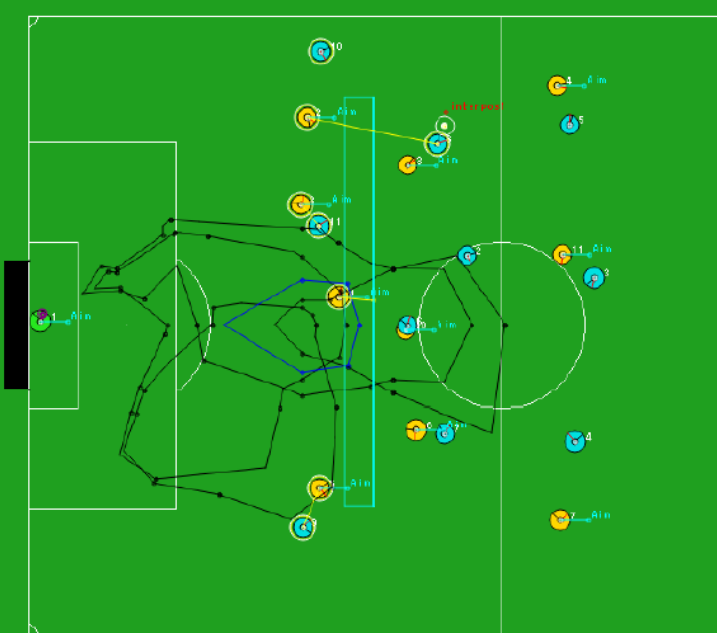
\includegraphics[scale=0.45]{images/wrightEagle_defensenet.png}
    \caption{WrightEagle's defensive net. The blue area represents the area to be defended and the blacks, all calculated areas. Image from \cite{wrighteagle2014}.}
    \label{fig:defensenet}
\end{figure}

\begin{figure}[H]
    \centering
    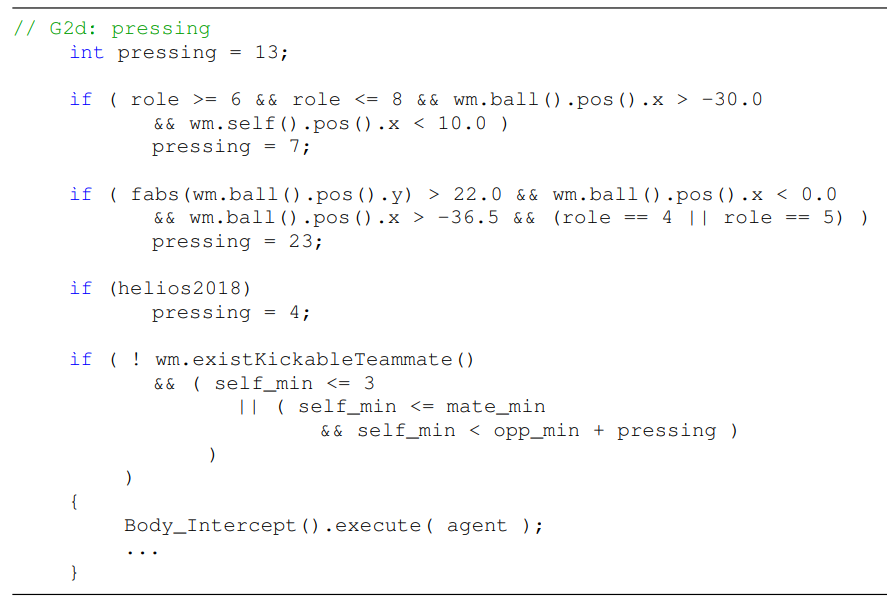
\includegraphics[scale=0.5]{images/gliders_pressing.png}
    \caption{Gliders' piece of code showing the fine tuning of pressing variable. Image from \cite{glidersv1}.}
    \label{fig:gliderscode}
\end{figure}

\section{Reinforcement Learning Agents}\label{section:RLAgents}
In this section we show some algorithms that introduced Reinforcement Learning into the SS2D. All teams here mentioned had a great performance in their years of competition.

\subsection{Brainstormers2d}
The pilot of Reinforcement and Deep Reinforcement Learning was Brainstormers2d. Since 2002 they invest in RL algorithms (\cite{brainstormers2002}) but here we mention only the techniques that gave them the first place in the competition: Intercept ball with RL and the NeuroHassle approach.
\subsubsection{Intercept Ball Task}
\cite{brainstormersIntercept} formalized their technique as a Markov Decision Process, \cite{bertsekas1996neuro}, where the State space was represented by the ball's velocity X and Y directions, agent's velocity X and Y directions, the distance between the agent and the ball and the relative angle between ball and agent. The actions available to the agent were turn and dash commands. They discretized the Environment Space into a grid of \num{6e5} cells. They also considered a noise-free environment to do the experiments.

As \cite{brainstormersIntercept} say, the technique outperformed their previous NI'02 Intercept Model and takes only one more cycle to intercept the ball then the Model Based algorithm described in the paper.

\subsubsection{The NeuroHassle Approach}
Brainstormers did a disruptive job introducing Neural Reinforcement Learning in the Soccer Simulation 2D league in 2006. \cite{neurohassle} technique (it was develop in 2006 but the paper was only published in 2009) shows that a well modeled reinforcement learning system can outperform a deterministic one.
They restricted their state space into a 9 dimensions one considering:
\begin{itemize}
    \item Distance d between defender and the attacker
    \item Velocity (v$_x$ and v$_y$ component) defender
    \item Absolute value of the attacker’s velocity
    \item Position (b$_x$ and b$_y$ component) of the ball
    \item Defender’s body angle relative to the attacker’s position
    \item Attacker’s body angle relative to his direction towards the goal
    \item Value of the angle $\gamma = \angle GAD$ with G as position of the goal, A as position of the attacker, and D as the position of the defender
\end{itemize}
They put as actions a discretized space of 76 dimensions where the first 40 were the dash command  varying the power from -100 to 100 with a 5 step and the last 36 were turn command varying the angle from -180 to 180 with a 10 degree step.

To specialize the agent, they created a set of \textit{training situations} $S$ ($|S|=5000$ described in Figure \ref{fig:neurohassleTS} and defined four \textit{training regions} shown in Figure \ref{fig:neurohassleTR}.

\begin{figure}[H]
    \centering
    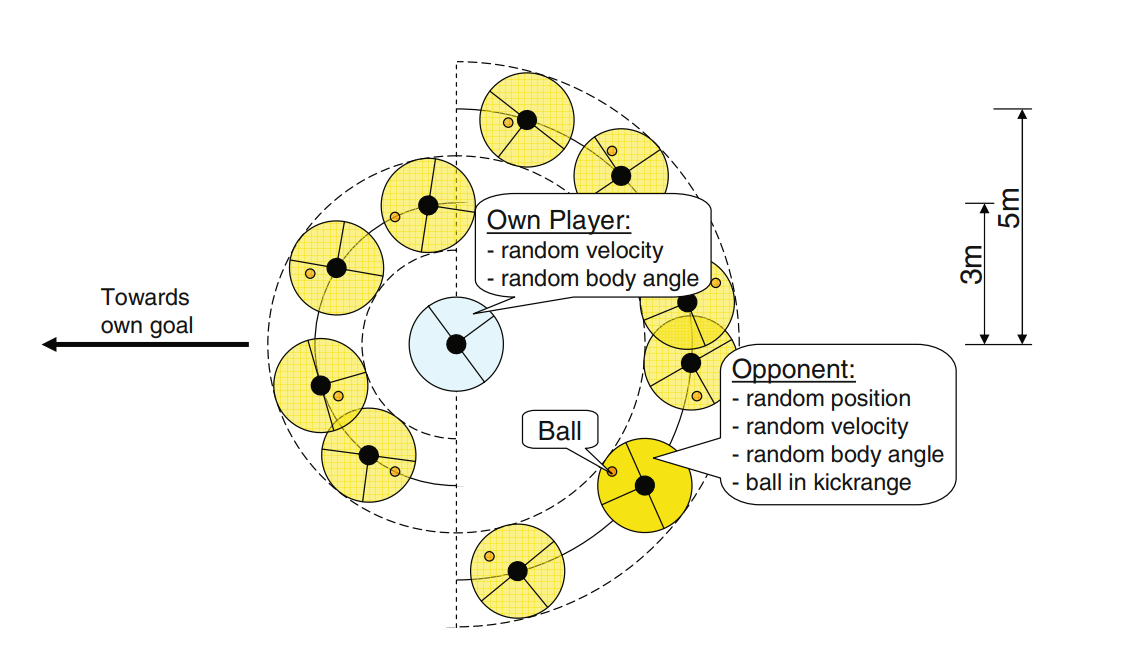
\includegraphics[scale=0.25]{images/neurohassleTS.png}
    \caption{Neurohassle's \textit{training situations}. Image from \cite{neurohassle}.}
    \label{fig:neurohassleTS}
\end{figure}

\begin{figure}[H]
    \centering
    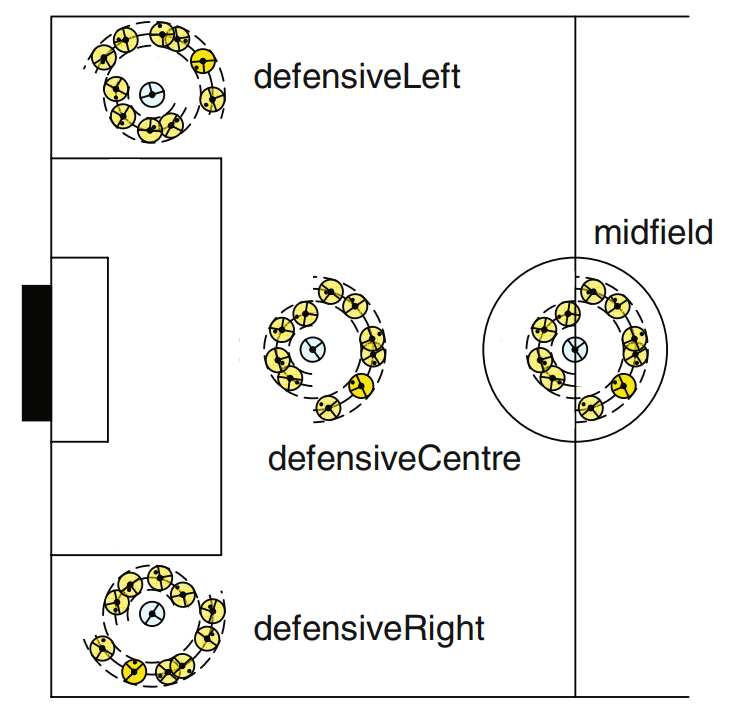
\includegraphics[scale=0.25]{images/neurohassleTR.png}
    \caption{Neurohassle's \textit{training regions}. Image from \cite{neurohassle}.}
    \label{fig:neurohassleTR}
\end{figure}

They did a simple reward function:
\begin{itemize}
    \item For each step without success: small negative reward 
    \item Failure: Large negative reward
    \item Success: Large positive reward
\end{itemize}

The Temporal Difference (TD) loss was calculated as follows:
\begin{gather*}
\label{eq1}
V(s_k) = (1-\alpha)*V(s_k) + \alpha*ret(s_k)
\\
ret(s_k) = \sum_{j=k}^{N} r(s_k, \pi(s_k))
\end{gather*}
Where $V(s_k)$ means the state value function, $ret(s_k)$ the summed rewards following state $s_k$ and $\alpha$ the learning rate. They employed a multi-layer perceptron (MLP) neural networks \cite{mlp} with a 9:18:1-topology to train the agent. See the results on Figure \ref{fig:neurohassleR1} and Figure \ref{fig:neurohassleR2}.

\begin{figure}[H]
    \centering
    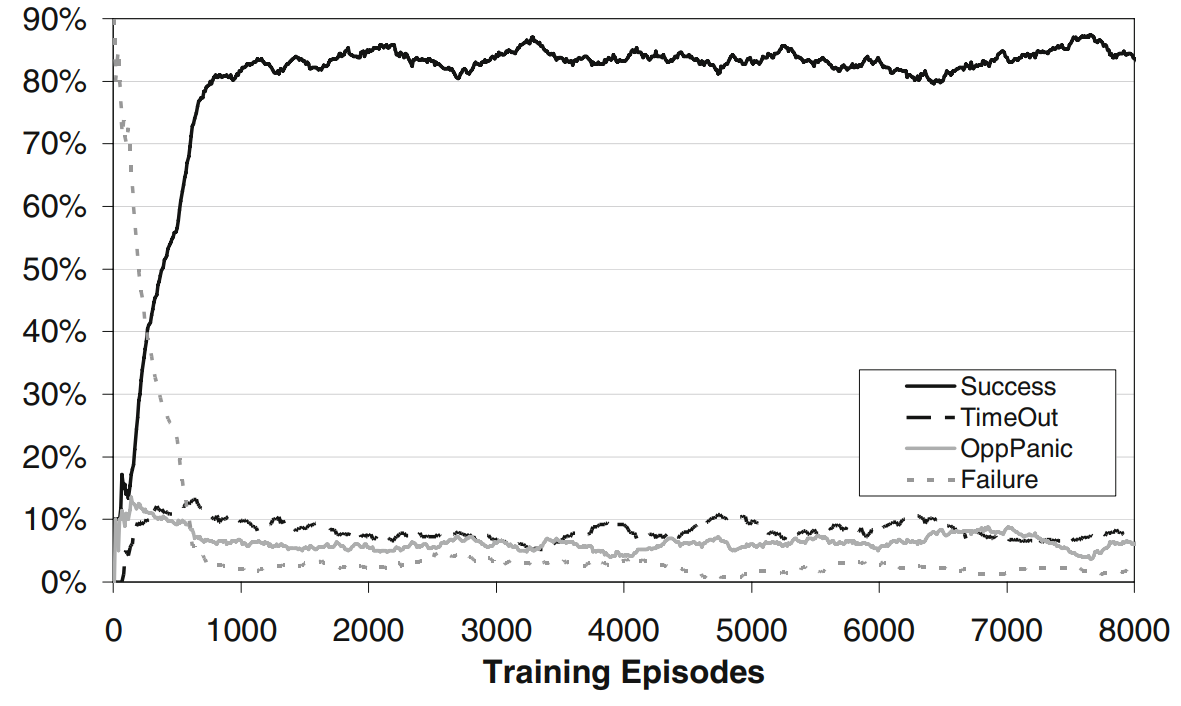
\includegraphics[scale=0.25]{images/neurohassleR1.png}
    \caption{Example of Learning Curve for Learning to Hassle. Image from \cite{neurohassle}.}
    \label{fig:neurohassleR1}
\end{figure}

\begin{figure}[H]
    \centering
    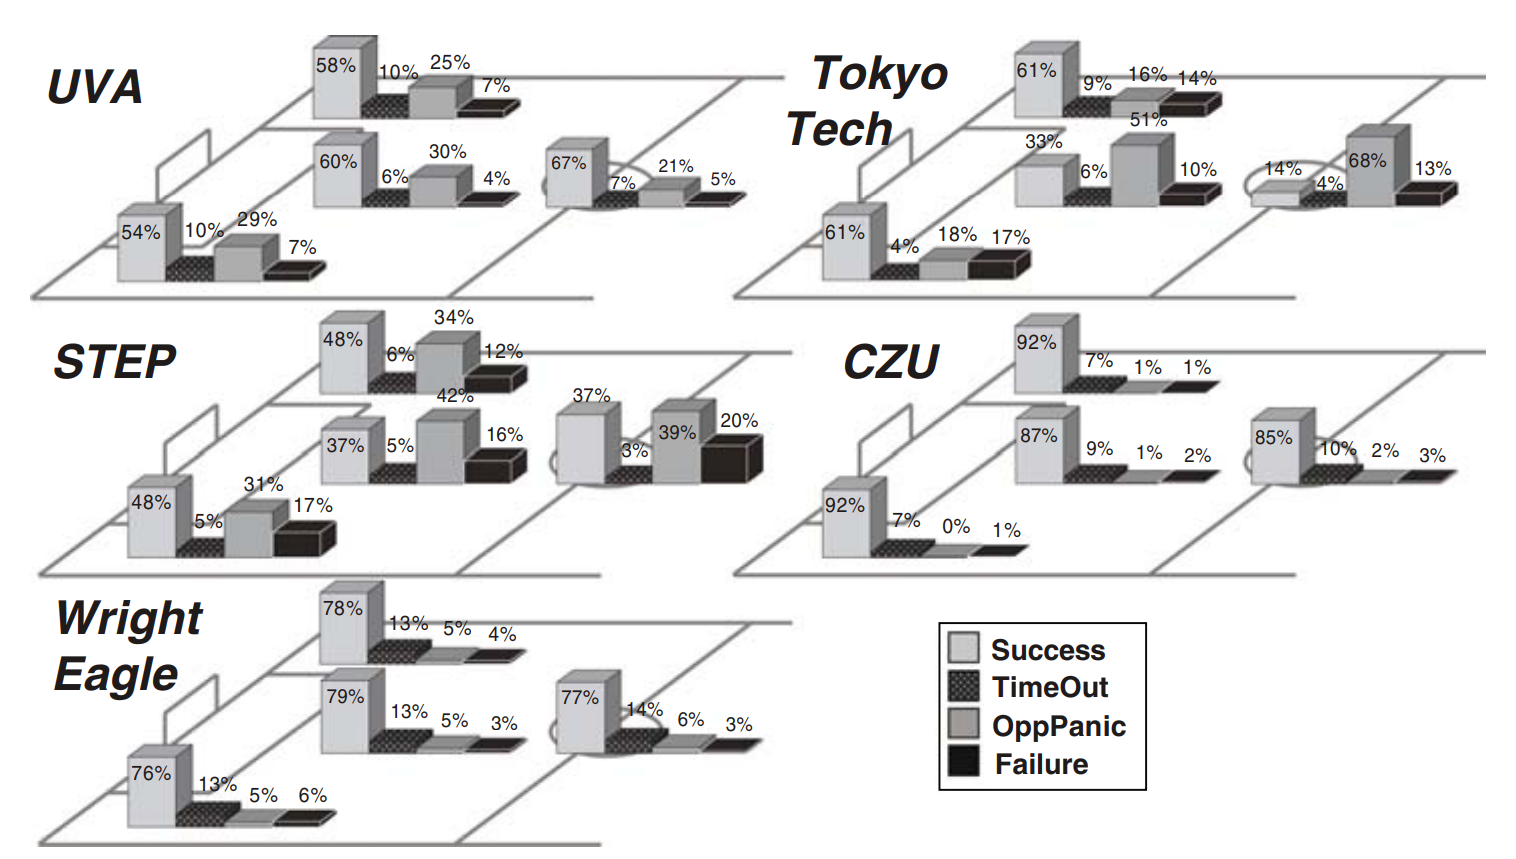
\includegraphics[scale=0.25]{images/neurohassleR2.png}
    \caption{\textit{Training regions} analysis for some teams from RoboCup2006. Image from \cite{neurohassle}.}
    \label{fig:neurohassleR2}
\end{figure}

\subsection{Cyrus2019}
\cite{cyrus} did an interesting job with a single agent cooperating with the goalie against an attacker. They did not specified the space features that they used, but they did tell us about \cite{hfo} environment, so we assumed that they used the high level state features from HFO. The actions they chose were block (\cite{cyrus2014}, a Cyrus' implementation of \cite{marlik2011}'s  Marlik block), intercept ball, cooperation with goalie (the defender ) and move (execute the movement according to the formation file). See Figure \ref{fig:cyrus_block}, \ref{fig:cyrus_intercept}, \ref{fig:cyrus_gassist} for the high level actions. 

\begin{figure}[H]
    \centering
    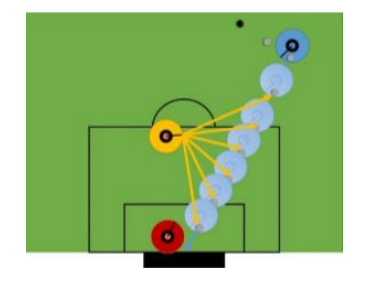
\includegraphics[scale=0.5]{images/cyrus_block.png}
    \caption{Cyrus' Block movement. Image from \cite{cyrus}.}
    \label{fig:cyrus_block}
\end{figure}

\begin{figure}[H]
    \centering
    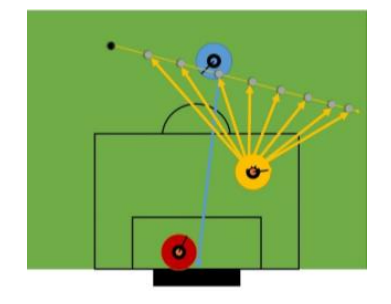
\includegraphics[scale=0.5]{images/cyrus_intercept.png}
    \caption{Intercept movement. Image from \cite{cyrus}.}
    \label{fig:cyrus_intercept}
\end{figure}

\begin{figure}[H]
    \centering
    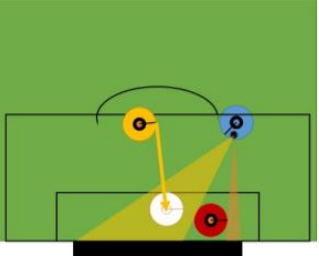
\includegraphics[scale=0.5]{images/cyrus_gassist.png}
    \caption{Cyrus' Goalie Assistant movement. Image from \cite{cyrus}.}
    \label{fig:cyrus_gassist}
\end{figure}

The reward modeling is described in Figure \ref{fig:cyrus_rewards}. They used a Deep Deterministic Policy Gradient (\cite{DDPG}) to train the agent with the TD function explained in Section \ref{section:ddpg}. The results are shown in Figure \ref{fig:cyrus_results}
\begin{figure}[H]
    \centering
    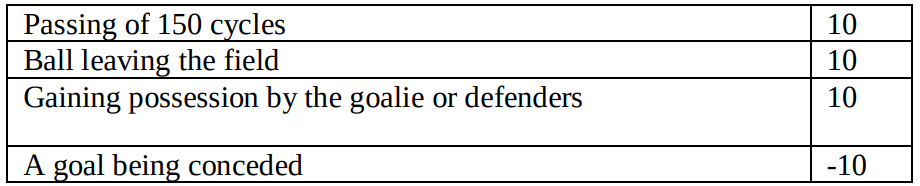
\includegraphics[scale=0.5]{images/cyrus_rewards.png}
    \caption{Cyrus' reward model. Image from \cite{cyrus}.}
    \label{fig:cyrus_rewards}
\end{figure}

\begin{figure}[H]
    \centering
    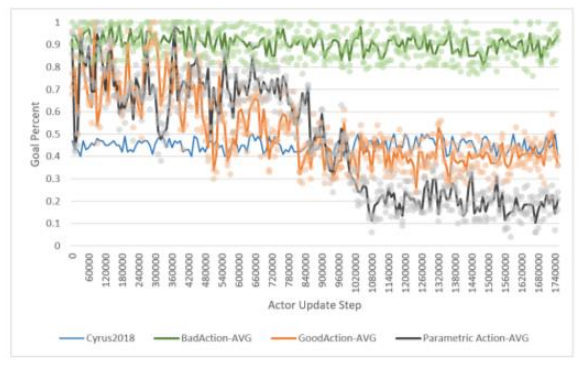
\includegraphics[scale=0.5]{images/cyrus_results.png}
    \caption{Cyrus' DDPG results. The best result is choosing a action and then CYRUS2018 (\cite{cyrus2018}) doing that action. Image from \cite{cyrus}.}
    \label{fig:cyrus_results}
\end{figure}